\documentclass[%
a4paper,%
10pt,%
oneside,%
DIV18,
headsepline,
plainheadsepline,
footsepline,
plainfootsepline,
%appendixprefix,
%automark,%
bibtotoc,%
liststotoc,%
BCOR12mm,%
halfparskip,%
openany,%
]{scrartcl}
\usepackage[utf8]{inputenc}
\usepackage[english]{babel}
\usepackage{float}
\usepackage{setspace}
\usepackage{mathpazo,courier}
\usepackage{listings,color}
\usepackage{courier}
\usepackage{tikz}
\lstset{basicstyle=\ttfamily\scriptsize}
\lstset{showspaces=false}
\lstset{showtabs=false}
\lstset{showstringspaces=false}
\lstset{keywordstyle=\bfseries}
\lstset{tabsize=4}
\lstset{frameround=ffff}
\lstset{extendedchars=true}
\lstset{stringstyle=\ttfamily}
\lstset{commentstyle=\ttfamily}
\lstset{backgroundcolor=\color[rgb]{0.92,0.92,0.92}}
%\lstset{numbers=left, numberstyle=\tiny, stepnumber=1, numbersep=5pt}
\lstset{captionpos=b}
\lstset{frame=single}
\setcounter{secnumdepth}{4} % Also numbering of \paragraph
\setcounter{tocdepth}{2} % Don't add \subsubsection to toc

% including and configuring package for links
\usepackage{hyperref}
\definecolor{darkblue}{rgb}{0,0,.5}

\hypersetup{pdftex=true, colorlinks=true, breaklinks=true, linkcolor=black, urlcolor=darkblue}

\title{Geany\LaTeX{} -- A \LaTeX{} plugin for Geany \\[1.5ex]
	   \normalsize Version 0.5dev}
\author{Frank Lanitz \\ \small{\href{mailto:frank@frank.uvena.de}{frank@frank.uvena.de}}}
\date{\today}

\newcommand{\up}[1]{\ensuremath{^\textrm{\scriptsize#1}}}

\begin{document}

\newpage
\dedication{\normalsize \textbf{Note:} Please note the document has been created on
\today. If you are using devel version from SVN, please compile and check
\texttt{doc/geanylatex.tex} from sources. Please check page \pageref
{sec:compiling_of_documentation}, section \ref{sec:compiling_of_documentation} how to do so. }

\pagenumbering{Roman}
\maketitle
\tableofcontents
\listoftables
\newpage
\pagenumbering{arabic}
\section{About the plugin}

Geany\LaTeX{} is a little plugin to improve support of \LaTeX{} on Geany.
It implements a couple of maybe useful functions:

\begin{itemize}
	\item Wizard to create new \LaTeX{} documents in a fast and easy way
	 	  with a bunch of templates available
	\item A front end for add labels \textbackslash label{} and
		  references \textbackslash ref{} and \textbackslash pageref{}
   		  with getting suggestion from aux file of document
	\item Inserting special characters through menu
	\item Help entering the right fields for BibTeX entries by
		  providing templates
	\item Easy inserting format patterns like \textbackslash texttt{}
		  through menu
	\item Support on inserting environments by offering an dialog and
		  recognising selections
	\item Shortcuts for inserting \textbackslash item and
		  \textbackslash newline
	\item Toolbar with often used format options
\end{itemize}

\section{News}
\subsection*{Since 0.4}
\begin{itemize}

	\item Introducing custom templates for \LaTeX-Wizard
	\item Adding a icon for \LaTeX-Wizard to toolbar
	\item Adding shortcuts for inserting common list environments
		  like \texttt{enumerate}, \texttt{itemize} and
		  \texttt{description}
	\item Some general bugfixes and improvments. As always, see
		  ChangeLog or svn log.
	\item Switch to waf for building the plugin
\end{itemize}

\subsection*{GeanyLaTeX{} 0.4 -- 2009-05-26}
\begin{itemize}
	\item Adding a toolbar with often used format commands
	\item Adding a configuration dialog to configure basic options of plugin
	\item Moved documentation into a \TeX{}-document
	\item Replace \textbackslash{}u-UTF-8 letters by octal coded chars to
		  don't depend on C99 anymore.
	\item Added a function to bulk replace special characters
    	  inside marked text by keybinding
	\item Added a function to replace special characters on typing
\end{itemize}

\section{Requirements}

\small{\textbf{Please note:} This section of documentation is only valid with standalone distribution of Geany\LaTeX{}. If you are planning to use the common geany-plugins project, please check documentation over there as there are some specialties you might like to know.}

For compiling the plugin yourself, you will need the GTK ($>= 2.8.0$)
libraries and header files. You will also need its dependency
libraries and header files, such as Pango, Glib and ATK. All these
files are available at \url{http://www.gtk.org}.

And obviously, you will need to have Geany with its header files
installed (in case you are compiling the plugin on your own). If you
have Geany installed from the sources, you should be ready to go. If
you used a prepared package e.g. from your distribution you probably
need to install an additional package, this might be called geany-dev
or geany-devel. Please note that in order to compile and use this
plugin, you need Geany 0.17 or later (Geany Plugin API v147 or higher).

Furthermore you need, of course, a C compiler and python installed. The
GNU version of the C compiler is recommended. Also there should be a
working \LaTeX-environment on your System.

There is no special need in RAM or CPU so the plugin should compile and
run on all systems Geany is able to run.

\section{Installation}

\small{\textbf{Please note:} This section of documentation is only valid with standalone distribution of Geany\LaTeX{}. If you are planning to use the common geany-plugins project, please check documentation over there as there are some specialties you might like to know.}

\subsection{Compiling the plugin itself}
Compiling and installing the code is done by the following three
commands:

\begin{figure}[h!]
\begin{lstlisting}
$ ./waf configure
$ ./waf build
$ ./waf install %$
\end{lstlisting}
\end{figure}

For more configuration details run \texttt{./waf --help}

By default the plugin is getting installed into the lib subfolder of
your found Geany installation. So if you have installed Geany to
\texttt{/usr/local/} the plugin will be installed to
\texttt{/usr/local/lib/geany/}. Translation files will be installed to
\texttt{/usr/local/share/locale/} in this case.

If there are any errors during compilation, check your build environment
and try to find the error, otherwise contact one of the
authors\footnote{Contact data can be found at chapter \ref{contact},
page \pageref{contact}.}

\subsection{Compiling of documentation}
\label{sec:compiling_of_documentation}
Sources of this documentation are available throught
\texttt{doc/geanylatex.tex} inside source tree. To compile the sources,
usage of \texttt{pdflatex} (should be delivered with your favorite
\LaTeX{} distribution) is recommended. For compiling into HTML format you
might like to use \texttt{htlatex}. The HTML version of this documentation
shipped with source tarball has been compiled with

\begin{figure}[h!]
\begin{lstlisting}
htlatex geanylatex.tex xhtml -cvalidate -interaction=batchmode
\end{lstlisting}
\end{figure}

\section{Usage}
\begin{figure}[h!]
	\centering{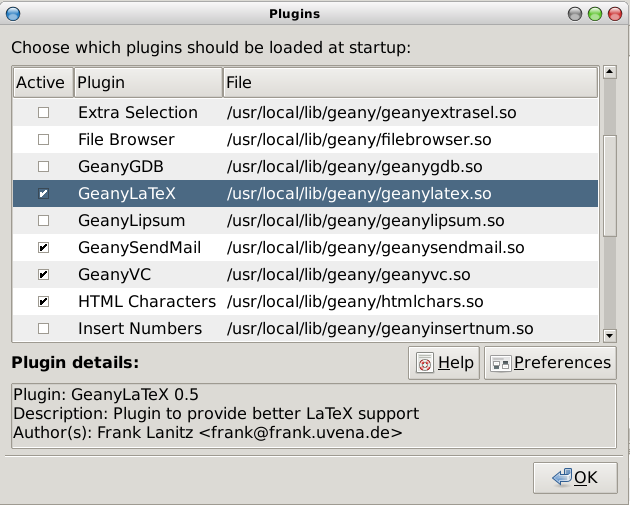
\includegraphics[height=7cm]{img/plugin_manager.png}}
	\caption{Plugin manager with Geany\LaTeX{} of Geany 0.16}
\end{figure}

After Geany\LaTeX{} has been installed successful the plugin can be
loaded through Geany's plugin manager and a new sub menu in the Tools
menu will appear as well as new key bindings will be available inside
Geany's key binding interface. Inside the sub menu you will find entries
for functions supported by this version of the plugin. The main menu entry
will be called something like \texttt{LaTeX}, depending on your locale.

Also if the option for showing the toolbar is activated on configuration
dialog, the toolbar with common used format functions appears on at top
of editor widget. This feature is turned off by default.


\section{Features}

Let's go into more detail on some features.


\subsection{\LaTeX-Wizard}

\subsubsection{General usage of wizard}
The \LaTeX-Wizard is implementing a easy way creating a number of
default documents.
\begin{figure}[h!]
	\centering{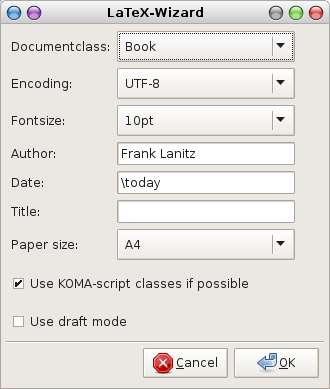
\includegraphics[height=7cm]{img/latexwizard.png}}
	\caption{\LaTeX-Wizard of version 0.4}
\end{figure}

The wizard is offering a chance to choose from a couple of templates 
with the possibility of adding customer templates. This can be 
chosen from \textbf{Templates} pulldown on top of dialog. 

This can be set by choosing the needed entry form
\textbf{Documentclass} pulldown menu.

\textbf{Encoding} is configuring the packages \texttt{inputenc} to
for example \texttt{\textbackslash usepackage[utf8]\{inputenc\}} in
case of the document encoding should be UTF-8. Also it sets the
encoding Geany is using for the newly created document.

\textbf{Font size} as well as \textbf{Paper size} will set class option
for font/paper size of the new created document. \textbf{Author},
\textbf{Date}, \textbf{Title} will be also passed to the corresponding
command inside the file header.

Option \textbf{Use draft mode} will add \texttt{draft} to list of
document options which allows some help during debugging of document.

Since KOMA script is quiet popular the option \textbf{Use KOMA script
if possible} allows to activate the usage of KOMA script. If this
options is activated instead of \texttt{book}, \texttt{scrbook} will
be used as document class. Default is activated here. This option is
deactivated by default and can be set through Geany\LaTeX{}'s
configuration dialog mentioned earlier in this document.

This wizard can also be called by a shortcut. Please have a look onto
section \ref{kb_latex_wizard}, page \pageref{kb_latex_wizard}.

\subsubsection{Default templates}
Document types that are currently supported by the wizard are:
\begin{itemize}
	\item book
	\item report
	\item article
	\item letter (default letter class)
	\item presentation (\LaTeX{} beamer)
\end{itemize}

\subsubsection{Extending by own templates}
Geany\LaTeX{} is offering a way for extending the wizard by user 
defined templates. This templates will be stored inside the plugin 
configuration dir with file extension glt. For creating a 
customized template you will need to create a normal *.tex file and 
store it inside the directory. On most Linux systems this should be 
\texttt{\textasciitilde/.config/geany/geanyLaTeX/}. 

Inside your template you can refer to wizard's field by using some special 
strings which are:

\begin{table}[H]
\centering
\label{tab:symbols_in_custom_templates}
\caption{List of available symbols on custom templates}
\begin{tabular}{l|p{10cm}}
\textbf{Symbol} & \textbf{Usage}\\ \hline
\texttt{\{CLASSOPTION\}} & Will be replaced by the classoptions set on 
	the wizard as for example font size or paper size.\\
\texttt{\{DOCUMENTCLASS\}} & Will be replaced by the choosen document 
	class based on the pulldown of wizard and whether option for KOMA 
	script has been set. \\
\texttt{\{DATE\}} & Will be replaced by the input given on the date 
	field of wizard.\\
\texttt{\{TITLE\}} & Will be replaced by the input given on the title 
	field of wizard.\\
\texttt{\{AUTHOR\} }& Will be replaced by the input given on the author 
	field of wizard.\\
\texttt{\{ENCODING\}} & Will be replace by choosen encoding from pulldown 
	of wizard\\
\texttt{\{OPENING\}} & Will be replaced by »Dear Sir or Madame« in local 
	geany\LaTeX{} is running with. If you like to overwrite it, please 
	don't use the symbol and hardcode the phrase instead.\\
\texttt{\{CLOSING\}} & Will be replaced by »With kind regards« in local 
	geany\LaTeX{} is running with. If you like to overwrite it, please 
	don't use the symbol and hardcode the phrase instead.\\
	\end{tabular}
\end{table}

If you have other than the default templates defined they will be 
add to templates pulldown. So when creating a template, please keep 
care to set up a good name for the file, as the filename will be 
the identifier you can choose from on pulldown. 

\subsection{Inserting References and Labels}
An often used feature on writing of documents is adding and referring
to labels. Geany\LaTeX{} is adding some support here for more
comfortable adding new labels and reference offering a GUI.

\begin{figure}[h!]
	\centering{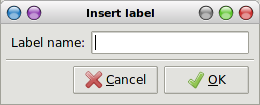
\includegraphics[height=2.5cm]{img/insert_label.png}}
	\caption{Insert label dialog on Geany\LaTeX{} 0.4}
\end{figure}

After an label was added Geany\LaTeX{} is offering a dialog for
inserting normal references and page references to an label.

\begin{figure}[h!]
	\centering{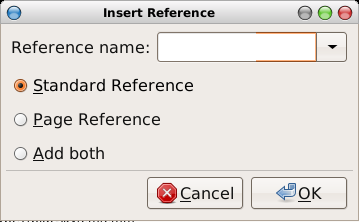
\includegraphics[height=3.5cm]{img/insert_reference.png}}
	\caption{Insert reference dialog on Geany\LaTeX{} 0.4}
\end{figure}

The suggestions inside the pull down are based on the aux files creating
by processing of *.tex file located inside directory of current \TeX-file.
When first step was successful the files are parsed for \texttt{\textbackslash
newlabel\{\}\{\}\{\}} and outcome is tried to interpret them properly.
The found entries will be inserted into pull down sorted by alphabet.

Both, the inserting labels as well as the inserting reference dialog
can be accessed by key binding also. See chapter \ref{kb_insert_label}
and \ref{kb_insert_reference} here.

\subsection{BibTeX templates for catalogue entries}
Geany\LaTeX{} is offering a number of often used templates for BibTeX
catalogue entries. They can be access by the plugin submenu in Geany's
tools menu:
\begin{itemize}
	\item Article
	\item Book
	\item Booklet
	\item Conference
	\item Inbook
	\item Incollection
	\item Inproceedings
	\item Manual
	\item Mastersthesis
	\item Misc
	\item PhdThesis
	\item Proceedings
	\item Techreport
	\item Unpublished
\end{itemize}
When choosing an entry from list on menu a templace with common used
fields will be generated and inserted into the document.
The template will be inserted on position of cursor which will
no be moved during the process. As an example for a book, this will be
inserted to the document:

\begin{figure}[h!]
\begin{lstlisting}
@Book{
Author = {},
Editor = {},
Publisher = {},
Title = {},
Year = {},
}
\end{lstlisting}
\end{figure}

\subsection{Replacement of special characters}
Geany\LaTeX{} is able to replace special characters to their there \TeX\
substitute. This can be done in two different ways:

\begin{enumerate}
	\item \textbf{On input:} If this switch is active all special
		  characters will be replaced during typing of text. You can
		  turn the switch on/off at Replacement of special characters
		  submenu inside.
	\item \textbf{Bulk replace of selected text:}
		  A selected text will be parsed and all known special characters
		  will be replaced by their \TeX{} substitute. This can be very useful
		  on importing a large amount of text into your document
		  including characters like ö or \frqq. This function is
		  available through the Replacement of special characters
		  submenu on plugin's submenu of Geany's Tools menu.
\end{enumerate}

For both functions there are also shortcuts available.

\subsection{Inserting of special character}
The plugin is offering a number of special characters with their \TeX{}
substitutes to be inserted on easy accessing through the plugin menu.

\subsection{Inserting of Environment}
Geany\LaTeX{} is offering a feature for inserting environments into your
documents. It can be chosen from a pulldown menu and will be inserted at
current position of cursor. If there is a selection activ, the selection
will be included into environment.

\begin{figure}[h!]
\begin{lstlisting}
\begin{your_environment}
	% ... selected text ...
\end{your_environment}
\end{lstlisting}
\end{figure}

In case of an empty (= no selection) an empty environment with
\begin{figure}[h!]
\begin{lstlisting}
\begin{your_environment}
...
\end{your_environment}
\end{lstlisting}
\end{figure}

will be inserted to the document.

\begin{figure}[h!]
	\centering{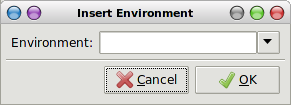
\includegraphics[height=2.5cm]{img/insert_environment.png}}
	\caption{Insert environment dialog on Geany\LaTeX{} 0.4}
\end{figure}


\subsection{Format}
Geany\LaTeX{} is able to help on formation of text. For doing this its
offering you to insert often use format patterns to your document.
Patterns that are currently supported are:

\begin{itemize}
	\item Italic
	\item Boldfont
	\item Underline
	\item Slanted
	\item Typewriter
	\item Small Caps
	\item Emphasis
	\item Centered
	\item left-aligned
	\item right-aligned
\end{itemize}

Geany\LaTeX{} will add the correct format pattern to the document. If
there is an selection active, that pattern will be placed around so
the selected text will be formatted with this chosen style.

Following items are also accessible using the Geany\LaTeX{} toolbar:
\begin{itemize}
	\item Italic
	\item Boldfont
	\item Underline
	\item Centered
	\item left-aligned
	\item right-aligned
\end{itemize}

\section{Configuration}

GeanyLaTeX{} can be configured in two major ways:
\begin{enumerate}
\item GeanyLaTeX{}'s configuration dialog
\item Geany's keybindings interface
\end{enumerate}

\subsection{GeanyLaTeX{}'s configuration dialog}
With version 0.4 the configuration dialog is offering two options which
can be changed:

\subsubsection{Use KOMA script by default}
KOMA script bei Markus Kohm is a very popular set of document classes
mainly used in Europe. With this option the default setting for e.g.
\LaTeX{}-Wizard can be configured\footnote{Currently only position where
this option is being used to be honest}. Option is turned off by default.

\subsubsection{Show extra toolbar}
Decides whether toolbar with some format icons should appear in the top
of editor widget. Option is turned off by default. Just give it a try.

\subsection{Key bindings}
Keybindings which are available:

\begin{table}[H]
\caption{List of available keybindings}
\centering
\label{kb_latex_wizard}\label{kb_insert_label}\label{kb_insert_reference}
\label{kb_toggling_input_replacement} \label{kb_replacement_of_special_char}
\begin{tabular}{l|p{9cm}}
\textbf{Shortcut} & \textbf{Description} \\ \hline\hline
Run LaTeX-Wizard & Starts the LaTeX-Wizard for creating a new document\\ \hline
Insert \textbackslash label & Runs the dialog for inserting a new label into your document. \\\hline
Insert \textbackslash ref & Starts an dialog for easy inserting \texttt{\textbackslash ref} and\texttt{\textbackslash pageref} into your document. The dialog is supporting easy parsing of aux files so it can suggest a couple of already set labels.\\\hline
Insert linebreak \textbackslash \textbackslash & Inserts a a newline \textbackslash{}\textbackslash{} into the document.\\\hline
Turn input replacement on/off & A shortcut for turning input replacement on or off. When input replacement is activated special characters like \v{e} are replaced by there \TeX{} substitute like \texttt{\textbackslash{}v\{e\}}\\\hline
Replacement of special characters & A selected text will be parsed and all known special characters
will be replaced by their \TeX{} substitute. This can be very useful on importing a large amount of
text into your document including characters like ö or \frqq. \\\hline
Run insert environment dialog & Runs a dialog for easy inserting an environment. If there is some text
selected, the environment will be placed around.\\\hline
Insert \textbackslash item & This shortcut will add an simple \textbackslash item to the document.
This can be very useful during writing of lists with a huge number of
items.\\\hline
Format selection in bold font face & Format a selection with bold font face.
This is done be adding \texttt{\textbackslash textbf\{...\}} around selection. \\\hline
Format selection in italic font face & Format a selection with italic font face.
This is done be adding \texttt{\textbackslash textit\{...\}} around selection.\\\hline
Format selection in typewriter font face & Format a selection with typewriter
font face. This is done be adding \texttt{\textbackslash texttt\{...\}} around
selection.\\\hline
Format selection centered & Formats selected text centered on page (uses \texttt{\textbackslash{}centering} \\\hline
Format selection left-aligned & Formats selected text left-aligned on page (uses \texttt{\textbackslash{}raggedleft} \\\hline
Format selection right-alignedm & Formats selected text right-aligned on page (uses \texttt{\textbackslash{}raggedright}\\\hline
Insert description list & Inserts an description environment as well as a 1\up{st} \textbackslash{}item element.\\\hline
Insert itemize list & Inserts an itemize environment as well as a 1\up{st} \textbackslash{}item element.\\\hline
Insert enumerate list & Inserts an enumerate environment as well as a 1\up{st} \textbackslash{}item element.\\\hline

\end{tabular}
\end{table}

\newpage
\section{Donating to the plugin}
If you like the plugin, there are a number of ways, how to donate the
development of the plugin.

\subsection{Extending plugin}

\subsubsection{Adding a new translation}
\label{sec:translating}
Currently the plugin is available in English and German language but
we are always looking for other translations to. There are two major
topics in translation:

\begin{enumerate}
\item \textbf{Translation of plugin:}
	   Adding a new translation and improving an existing one is easy to
	   do. After catching the source tarball and extracting you can find
	   all needed files inside the po folder. \\
	   Please contact the authors if you plan to update/add a translation
	   to ensure nobody else is currently working on and avoid double
	   work and to get some further information about translation (see
	   chapter \ref{contact}).
\item \textbf{Translation of documentation:}
	   Since this document is currently only available in English it
	   would be helpful for not English speaking people to have a
	   translated version. If you like to do an translation, please
	   also contact one of the authors for details (see chapter \ref{contact}).
\end{enumerate}

\subsubsection{Adding a new feature}
New features are always highly welcome. The TODO file inside source
code archive gives a good idea of current wished features and which
are being worked on. Also you can have a look onto the feature request
tracker of geany-plugins project at
\url{http://sourceforge.net/tracker/?group\_id=222729} whether you find
something interesting. Of course we are also open for not in the
sources mentioned before listed items. Just contact one of the authors
(see chapter \ref{contact}).

\subsection{Testing \& bug reporting}
Geany\LaTeX{} is tested mainly on x86 and x86\_64 architecture running
GNU/Linux. Also it was tested on some Windows 32 versions like XP SP3
very briefly. Since there are also other systems available, testing on other
platforms and maybe reporting of issues is highly appreciate.

\subsection{Packaging}
Geany\LaTeX{} is part of the geany-plugins project even though there
are releases independent of a major release of the project. Therefor
there are two things you can do here:
\begin{enumerate}
	\item Package the plugin for your operating system or
	distribution. As you might can imagine, the authors unfortunately
	cannot support all possible platforms.
	\item Help to keep releases and packages of geany-plugins project
	up to date for current version of Geany.
\end{enumerate}

\subsection{Improving and extending of documentation}
Documentation is never complete. There are spelling mistakes,
paragraphs that needs to be extended or rewritten because they are not
clear or topics that were missed out at all.

The documentation is written in \LaTeX{} so all you need is to get the
tex file from doc folder and add or update the content.
After this, just send a diff or complete file to one of the authors.

\subsection{Propaganda}
And of course, tell others of Geany and this plugin. If you like to do
a talk about Geany\LaTeX{} and/or Geany in general, there is some code
available on \url{http://git.geany.org/talks/} you might can use as a
start point for preparing your own presentation. If your favourite
language is not yet available there, please feel free to do your own
translation and in best case send your translation to one of
Geany's\footnote{Check for addresses \url{http://www.geany.org}}
development team so it can be added to archive.


\section{Development}
\subsection{Development version}
You can checkout the current source code from the Subversion repository
at Sourceforge.net. Get the code from:

svn checkout
http://geany-plugins.svn.sourceforge.net/svnroot/geany-plugins/trunk/geanylatex

\subsubsection{Sending a patch}
If you want to create a patch, please respect the license of
Geany\LaTeX{} as well as intellectual property of third. Patches that
should be included to the default distribution must be licensed under
the same conditions as Geany\LaTeX{} by the copyright owner.

\section{Known issues}
At time of the the documentation was created no issue were known.
Since this is only a snapshot, you will find more recent information
for all reported issues bug tracking system of SF at \\
\url{http://sourceforge.net/tracker/?group\_id=222729}

\newpage
\section{Recommendations to improve work with \LaTeX{} and Geany}
Geany is offering a number of nice features, that can be used to make
daily work more easy without need to write a new plugin or extend
Geany\LaTeX.

\subsection{Geany's code snippet function}
Geany is allowing you to define code snippets and inserting them easy
during writing a document. This gives you some more flexibility than to
create new commands.

A possible snippet for snippets.conf could be:

\begin{figure}[h!]
\begin{lstlisting}
[LaTeX]
frame=\\begin{frame}\n%ws%\\frametitle\n%ws%%cursor%\n\\end{frame}
block=\\begin{block}\n%ws%%cursor%\n\\end{block}
itemize=\\begin{itemize}\n%ws%\\item %cursor%\n\\end{itemize}
enumerate=\\begin{enumerate}\n%ws%\\item %cursor%\n\\end{enumerate}
description=\\begin{description}\n%ws%\\item %cursor%\n\\end{description}
\end{lstlisting}
\end{figure}

A snapshot of authors' last version for LaTeX can be found on
\url{http://www.geany.org/Download/Extras}

\subsection{Other useful plugins}
As mentioned before a number of useful functions were already
implemented with other plugins. Below you will find a list with the
authors's recommendations. More nice plugins can be found on Geany's
plugins page at \url{http://www.geany.org}.

\subsubsection{GeanyLipsum}
This plugin implements an easy way for inserting Lorem Ipsum text into
a document. The length of the inserted text if configurable so the
plugin can be very helpful on testing layout.\\
\textbf{Homepage:} \url{http://frank.uvena.de/en/Geany/geanylipsum/}

\subsubsection{geanyVC}
When working on bigger documents a version control system like
Subversion could be useful to keep versions. GeanyVC is adding a easy
to use frontend for a number of popular version controll systems such
as git, Subversion, CVS, Bazaar or Mercural.\\
\textbf{Homepage:} \url{http://plugins.geany.org/geanyvc/}

\subsubsection{tasks out of the addons plugins}
A plugin that is recognising \texttt{TODO} or \texttt{FIXME} tags
inside a document and allows to easy jump to these entries. This
function is similar to the \texttt{todo} package but doesn't require
recompiling of the document. Recognised tags will be inserted to
another tab in Geany's message widget.\\
\textbf{Homepage:} \url{http://plugins.geany.org/addons/}

\section{License}
Geany\LaTeX{} and all its parts is distributed under the terms of the
GNU General Public License as published by the Free Software
Foundation; either version 2 of the License, or (at your option) any
later version. A copy of this license can be found in the file COPYING
included with the source code of this program. If not, you will be
able to get a copy by contacting the Free Software Foundation, Inc.,
51 Franklin Street, Fifth Floor, Boston, MA 02110-1301, USA.


\section{Bugs, questions, homepage}
\label{contact}
If you found any bugs or want to provide a patch, please contact Frank
Lanitz (frank(at)geany(dot)org). Please also do so, if you got any
questions and visiting \\ \url{http://frank.uvena.de/en/Geany/geanylatex/}
didn't help you to figure out the answer. Visiting the website is also
a good start if you want to check for any update on this plugin.

\end{document}
